%!TEX root = ../book_ML.tex

\chapter{Ảnh màu}
\label{apd:color}

\begin{figure}[]
% caption on side
\floatbox[{\capbeside\thisfloatsetup{capbesideposition={right,top},capbesidewidth=7cm}}]{figure}[\FBwidth]
{\caption{
Ví dụ về 1NN. Các hình tròn khác màu thể hiện các điểm dữ liệu huấn luyện của các lớp khác nhau.  Các vùng nền thể hiện những điểm được phân
loại vào lớp có màu tương ứng khi sử dụng 1NN (Nguồn:
{K-nearest
neighbors algorithm  --  Wikipedia} (\url{https://goo.gl/Ba4xhX}), ảnh màu của Hình~\ref{fig:6_1nn_c}.).
}
\label{fig:6_1nn_c}}
{ % figure here
% 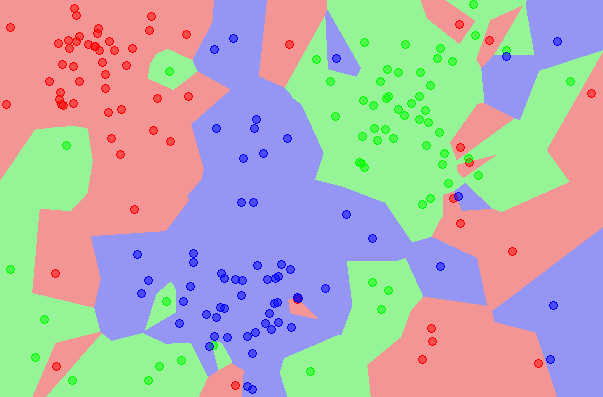
\includegraphics[width=.5\textwidth]{Chapters/03_SimpleML/6_knn/Map1NN.png}
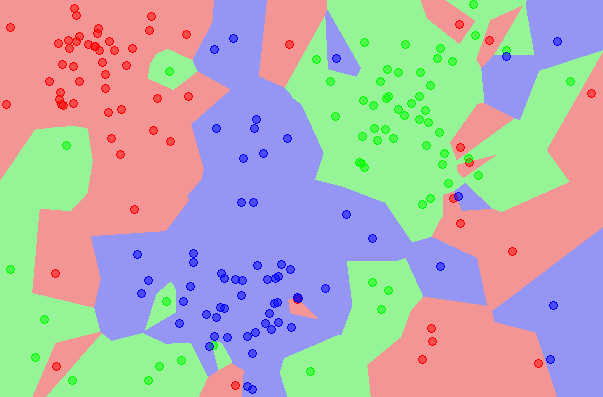
\includegraphics[width=.5\textwidth]{Chapters/03_SimpleML/6_knn/Map1NN.png}
}
\end{figure}



\begin{figure}[]
\centering
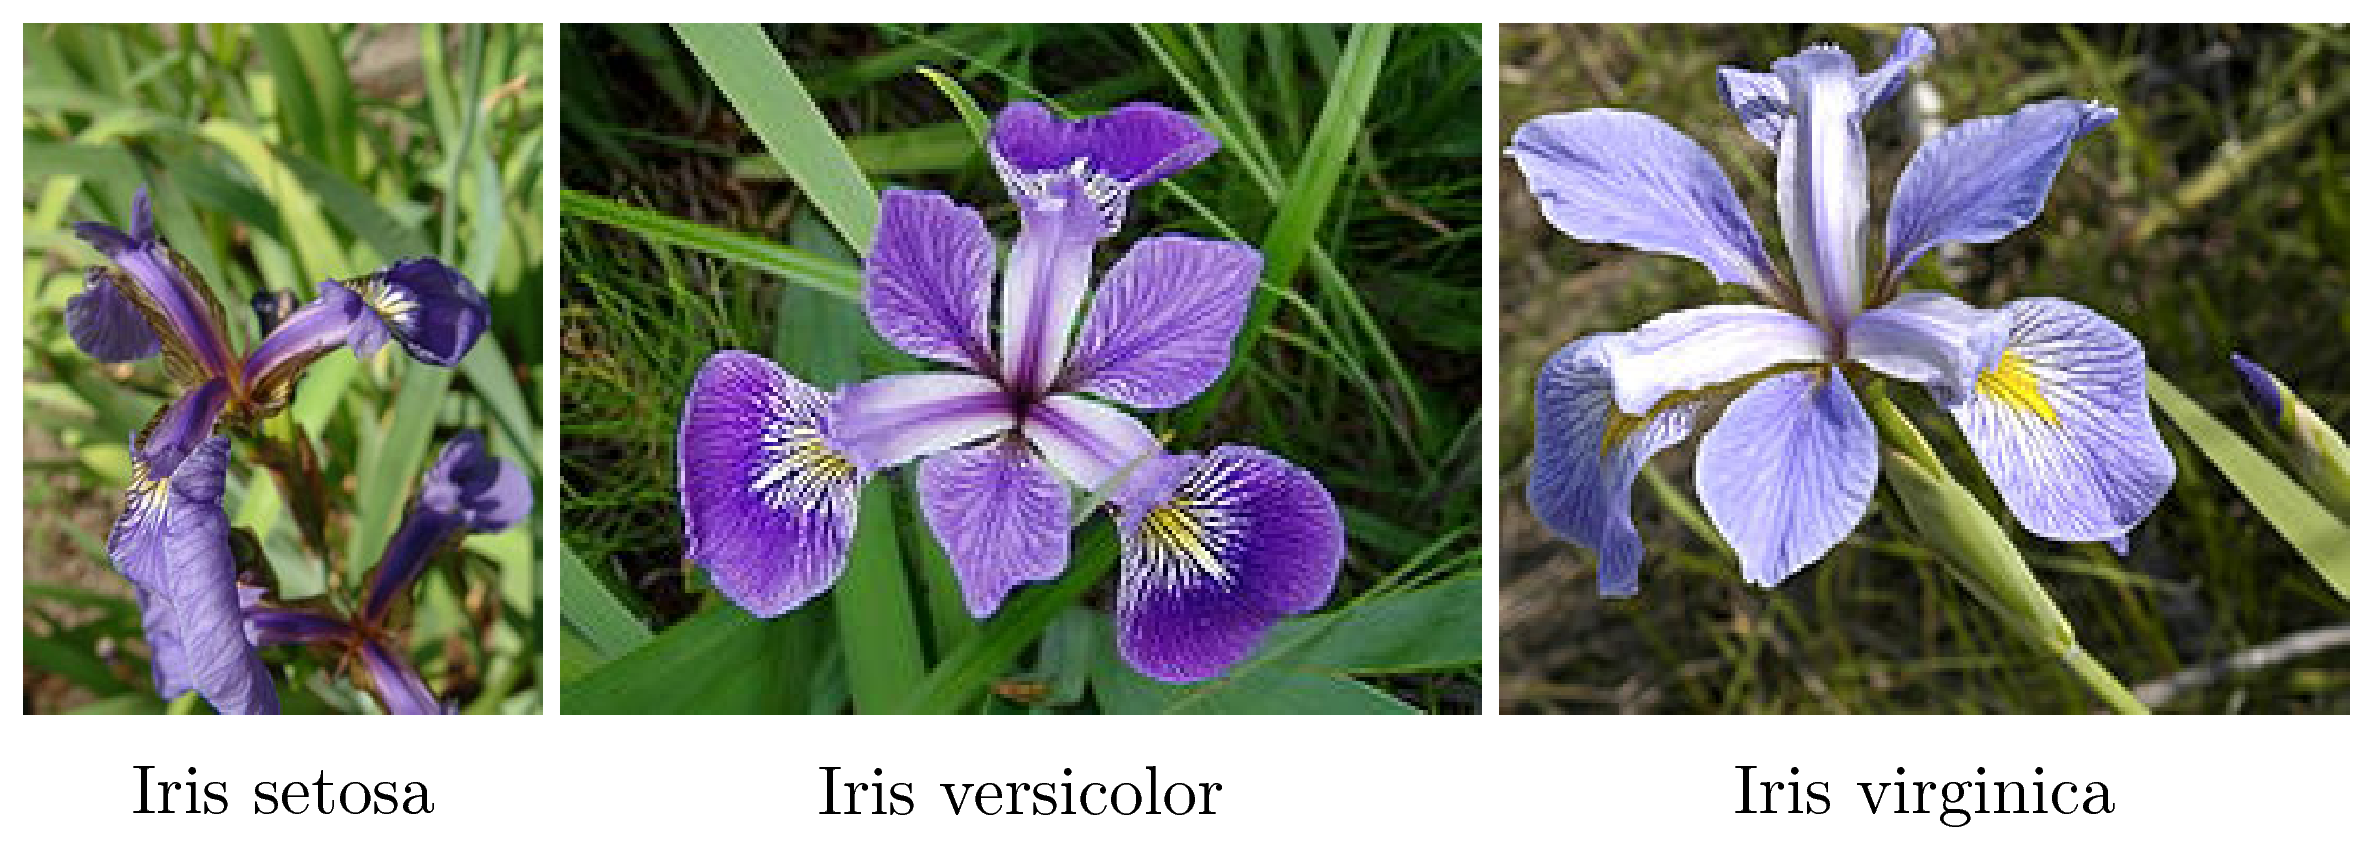
\includegraphics[width = \textwidth]{Chapters/03_SimpleML/6_knn/iris.png}
\caption[]{Ba loại hoa lan trong bộ cơ sở dữ liệu hoa Iris (ảnh màu của Hình~\ref{fig:6_iris}).}
\label{fig:6_iris_c}
\end{figure}

% ******************************************************************************
\begin{figure}[t]
% caption on side
\floatbox[{\capbeside\thisfloatsetup{capbesideposition={right,top},capbesidewidth=6cm}}]{figure}[\FBwidth]
{\caption{
\textit{Ảnh:Trọng Vũ} (\url{https://goo.gl/9D8aXW}, ảnh màu của Hình~\ref{fig:5_girl}) .
}
\label{fig:5_girl_c}}
{ % figure here
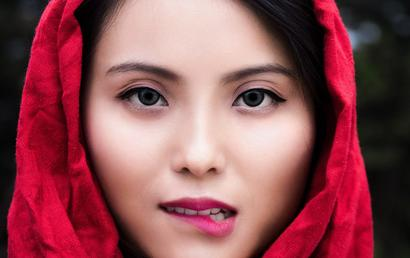
\includegraphics[width=.5\textwidth]{Chapters/03_SimpleML/4_kmeans/girl3.jpg}
% 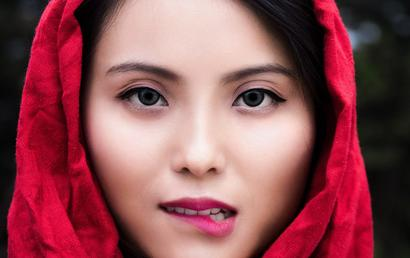
\includegraphics[width=.5\textwidth]{Chapters/03_SimpleML/4_kmeans/girl3.jpg}
}
\end{figure}
% ******************************************************************************
\begin{figure}[t]
% caption on side
\floatbox[{\capbeside\thisfloatsetup{capbesideposition={right,top},capbesidewidth=6cm}}]{figure}[\FBwidth]
{\caption{
Kết quả nhận được sau khi thực hiện phân cụm K-means cho các điểm dữ liệu.
Có ba cụm dữ liệu tương ứng với ba màu đỏ, hồng, đen (ảnh màu của Hình~\ref{fig:5_girl_seg}).
}
\label{fig:5_girl_seg_c}}
{ % figure here

\includegraphics[width=.5\textwidth]{Chapters/03_SimpleML/4_kmeans/girl_seg.png}
}
\end{figure}
% ******************************************************************************
\begin{figure}[t]
\centering
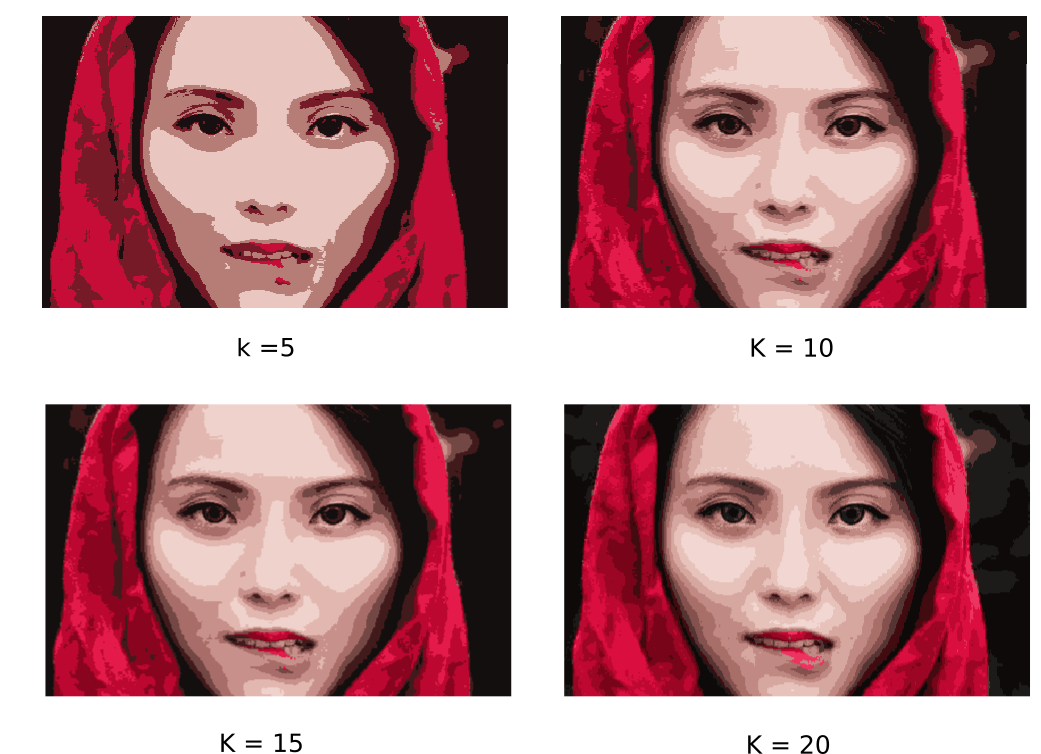
\includegraphics[width = \textwidth]{Chapters/03_SimpleML/4_kmeans/girl_all.png}
\caption[]{Chất lượng nén ảnh với số lượng cụm khác nhau (ảnh màu của Hình~\ref{fig:5_res}).}
\label{fig:5_res_c}
\end{figure}

% ******************************************************************************
\begin{figure}[t]
\centering
\floatbox[{\capbeside\thisfloatsetup{capbesideposition={right,top},capbesidewidth=6cm}}]{figure}[\FBwidth]
{
\caption{Đồ thị hàm sigmoid trong không gian hai chiều (ảnh màu của Hình~\ref{fig:10_logreg2db}).}
\label{fig:10_logreg2db_c}}
{
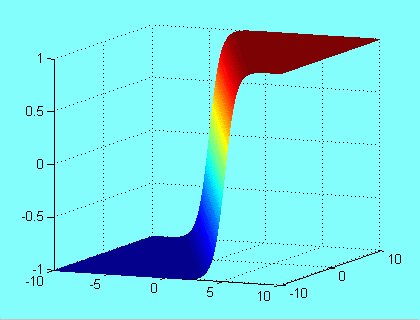
\includegraphics[width=.95\linewidth]{Chapters/05_NeuralNetworks/10_logisticregression/plaszczyzna.png}
}
\end{figure}

% ******************************************************************************


\begin{figure}[t]
\centering
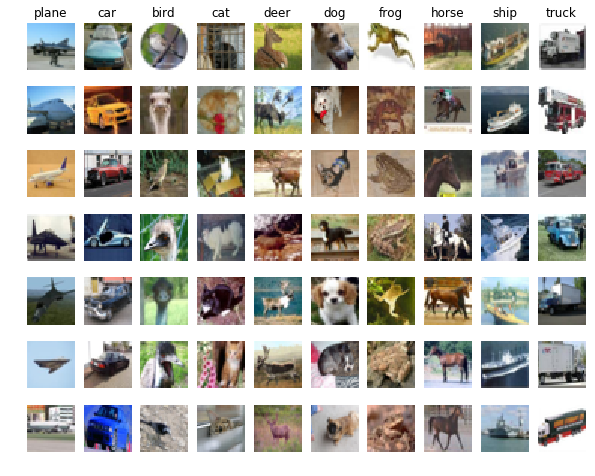
\includegraphics[width = \textwidth]{Chapters/09_SupportVectorMachines/22_multiclasssvm/cifar.png}
\caption[]{Ví dụ về các bức ảnh trong 10 lớp của bộ dữ liệu CIFAR10 (ảnh màu của Hình~\ref{fig:22_2}).}
\label{fig:22_2_c}
\end{figure}


% ******************************************************************************
\begin{figure}[]
\centering
% 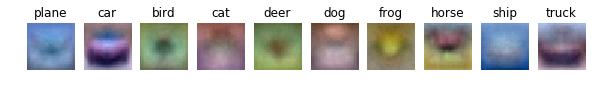
\includegraphics[width = \textwidth]{Chapters/09_SupportVectorMachines/22_multiclasssvm/learned_ws_2.png}
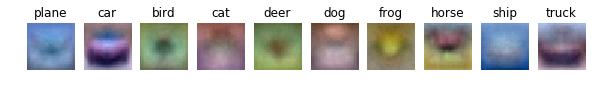
\includegraphics[width = \textwidth]{Chapters/09_SupportVectorMachines/22_multiclasssvm/learned_ws_2.png}
\caption[]{ Minh họa hệ số tìm được dưới dạng các bức ảnh (ảnh màu của Hình~\ref{fig:22_9_c}).}
\label{fig:22_9_c}
\end{figure}
% ******************************************************************************
